\chapter{Postprocessing tools\label{chap:postprocessing}}

Various tools are available to visualize gridded fields; some of them are presented in the following sections. We consider it is up to the user to utilize his favourite drawing tools for representing the numerical results. Nevertheless, we provide several basic tools to facilitate this task.


\minitoc

\section{Gnuplot\label{sec:visugnuplot}}
%-------------------------------------------

\index{Gnuplot}
\textsl{Gnuplot} is a free portable command-line driven interactive data and function plotting utility, available for various platforms (\url{http://www.gnuplot.info/}). We provide some routines for plotting \diva inputs and outputs (data, contour, mesh, analysis etc) with the help of this tool. Running \command{divagnu} makes plots in \texttt{png} format. 

\begin{tips}
Plots provided by \gnuplot are made to help the user to have a quick look at the results, immediately after the execution. However, these plots are not always suitable for publications or diffusion. The user is invited to create his own post-processing tools, for example appealing to the existing Matlab routines.
\end{tips}

\begin{tips}
If you need larger fonts, on some systems they are available and you can edit the plotting program \file{gnuwork$\backslash$divaplotall}
and replace the driver definition by
\begin{tiny}
\begin{verbatim}
echo set terminal png transparent giant font system 14 size 1920,1540 crop \#ffffff >> bidon
\end{verbatim}
\end{tiny}
\end{tips}

\begin{tips}
If you do not need all plots but only a few (eg. analysis, error and coastline) of them you can edit the plotting program \file{gnuwork$\backslash$divaplotall} and replace the script line \verb#for i in `ls diva_*`# 

by
\end{tips}

\verb#for i in diva_analysis diva_error diva_coastline#

\subsection{Installation}
%---------------------------

\gnuplot can be easily downloaded for windows systems on the web page \url{http://www.gnuplot.info}. For Cygwin users, there are two possibilities:

\begin{enumerate}

\item you do not have X Windows System installed: in this case, it is advised to only install \texttt{wgnuplot}, available at\\
\url{http://downloads.sourceforge.net/gnuplot/gp422win32.zip} for version 4.22.\\
Once you have downloaded it, just unzip the folder in the location of your choice (provided it is located on the path of your system). The \gnuplot\, window is activated either by typing \command{wgnuplot} in the Cygwin shell, or by creating a short-cut on your desktop to the executable \texttt{wgnuplot.exe}


\begin{figure}[htpb]
\centering
\parbox{.6\textwidth}{
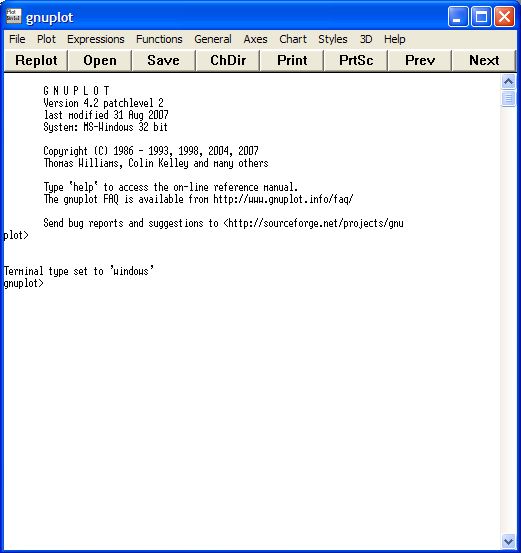
\includegraphics[width=.55\textwidth]{gnuplotwindows}
}\parbox{.4\textwidth}{
\caption{Gnuplot window.\label{fig:gnuplotwindows}}
}
\end{figure}

\item X Windows System is already installed: run again the Cygwin \command{setup.exe} (for downloading and updating your Cygwin installation); in the "Select Packages" screen, look for the "Math" entry, select \gnuplot\, and choose "`install". Once this installation is finished, \gnuplot\, is launched from a XWin (obtained after typing \texttt{startx}) window by typing \texttt{gnuplot}.

\begin{figure}[htpb]
\centering
\parbox{.7\textwidth}{
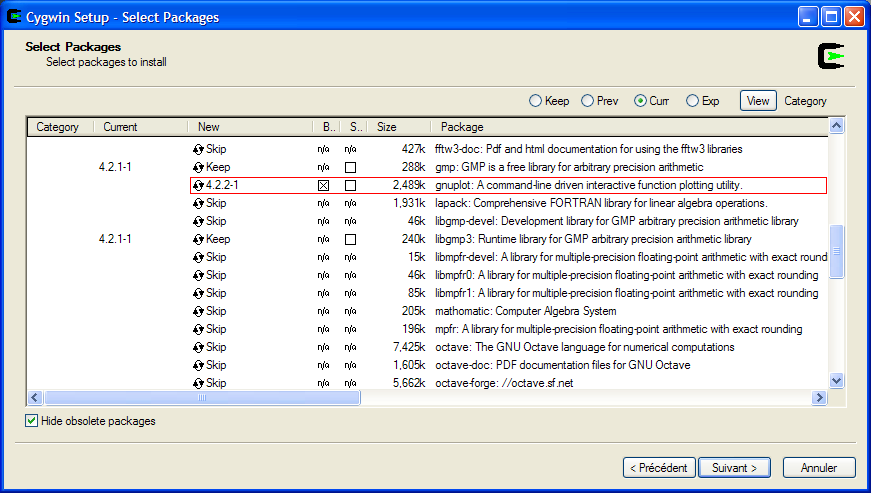
\includegraphics[width=.65\textwidth]{gnuplotinstall}
}\parbox{.3\textwidth}{
\caption{Installing \gnuplot\, with cygwin.\label{fig:gnuplotinstall}}
}
\end{figure}

\end{enumerate} 


\subsection{Utilization}
%-------------------------


Normally Fortran sources (\file{forgnuplot*.f}) have been compiled during the \diva installation and executables placed into \directory{DIVA3D/bin/}.

In directory \directory{divastripped/gnuwork/}, edit \command{divaplotall}  and adapt the header so that  \texttt{gplot} indicates the correct path to your \gnuplot executable.

\example\\
\begin{verbatim}
#====================================================
# ADAPT the following to the gnuplot executable
gplot=/cygdrive/c/cygwin/usr/gnuplot/bin/wgnuplot.exe
#====================================================
\end{verbatim}

From \directory{divastripped}, after running an analysis, type \command{divagnu}: this will create the figures in directory \directory{gnuwork/plots/}.
Note that \command{divagnu} will try to create all the possible figures, even if the corresponding script was not run, e.g., plot of outliers when no outlier detection was performed. This is why so many error messages are written on the screen, but you do not have to take them into account.
 %necessary for the plot inside the directory \texttt{./divastripped/gnuwork}

%From within gnuplot (Fig. \ref{fig:gnuplotwindows}): place yourself in the \texttt{gnuwork} directory and type:
%\begin{listevide}
%\item load 'gnuplotdata'
%\item load 'gnuplotcoast'
%\item load 'gnuplotcoastfilled'
%\item load 'gnuplotmesh' (mesh as triangles)
%\item load 'gnuplotmeshl'  (mesh with lines)
%\item load 'gnuplotanalysis'
%\item load 'gnuplotanalysissmooth'
%\item load 'gnuploterrorfield'
%\item load 'gnuplotuv'
%\end{listevide}
%
%These commands allow you to have a quick look at your data and results. In the file \texttt{gnuplotdata}, you might need to play with the value following the \texttt{ps} command (device dependent). 

Here are some examples of plots created with \gnuplot:

\begin{figure}[htpb]
\centering
\subfigure[Data and coastline]{
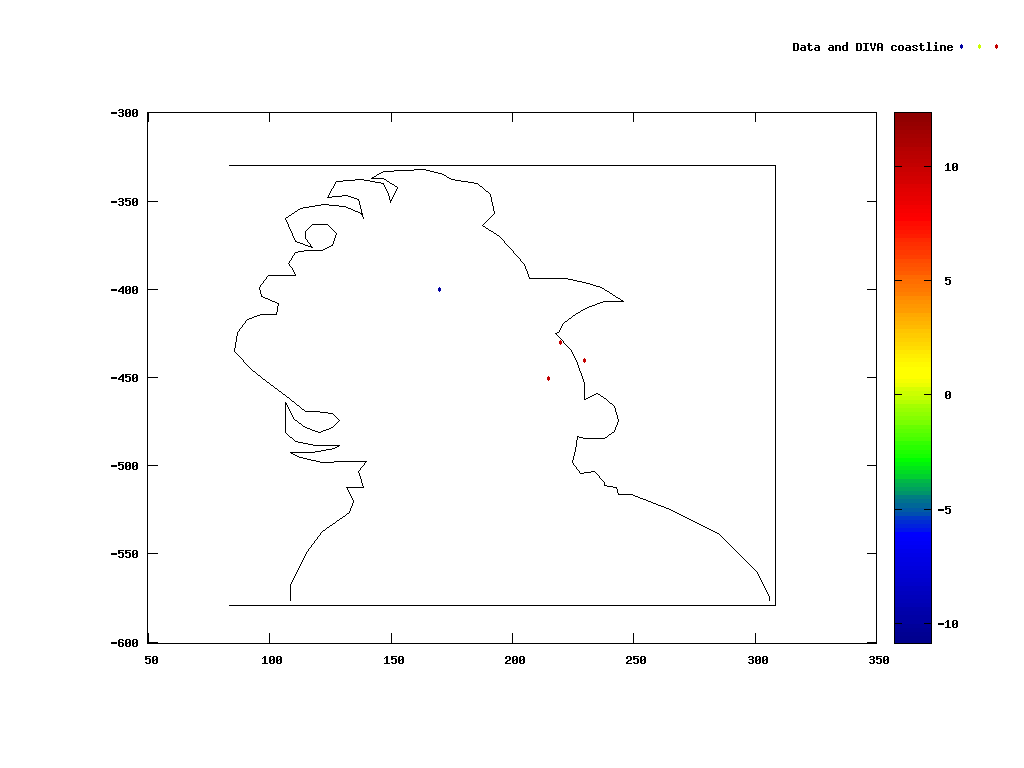
\includegraphics[width=.30\textwidth,height=.30\textwidth]{gnuplot_data_coast}
}\subfigure[Filled coastline]{
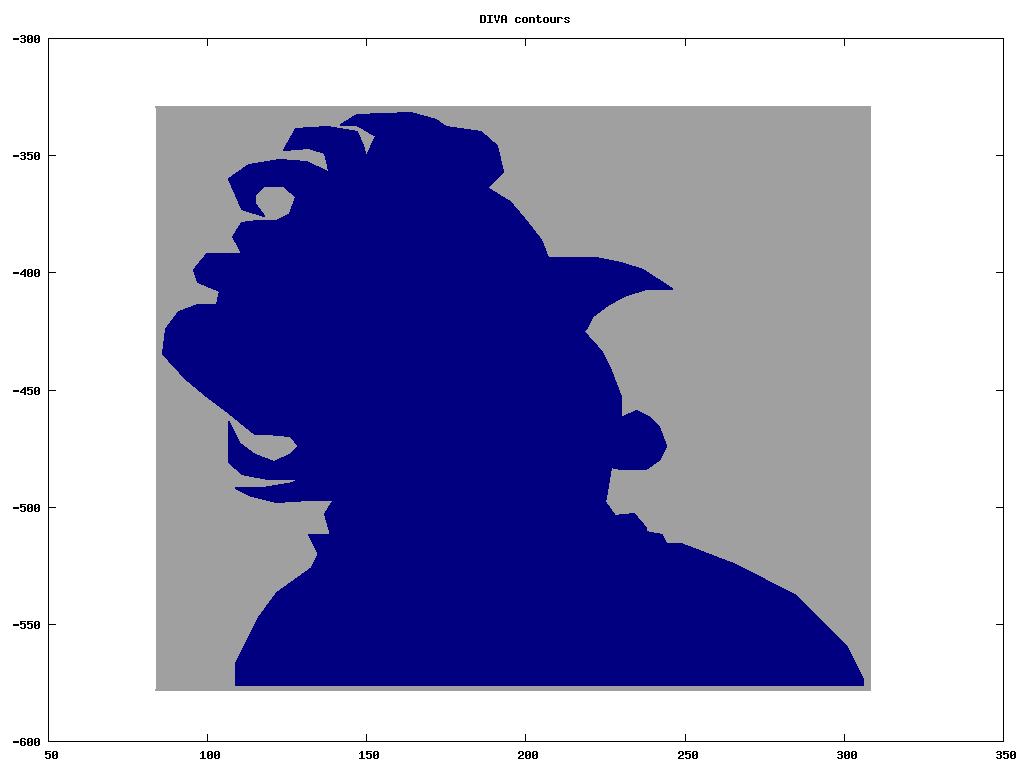
\includegraphics[width=.30\textwidth,height=.30\textwidth]{gnuplot_coastlinefilled}
}\subfigure[Mesh]{
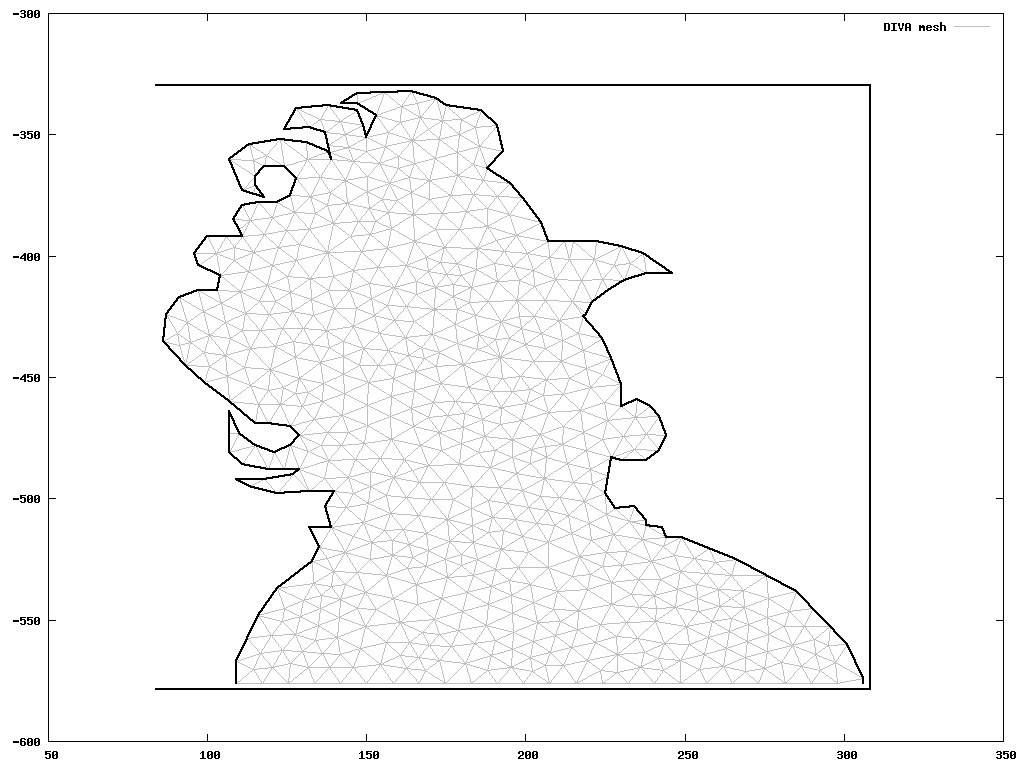
\includegraphics[width=.30\textwidth,height=.30\textwidth]{gnuplot_mesh}
}

\subfigure[Numbered mesh]{
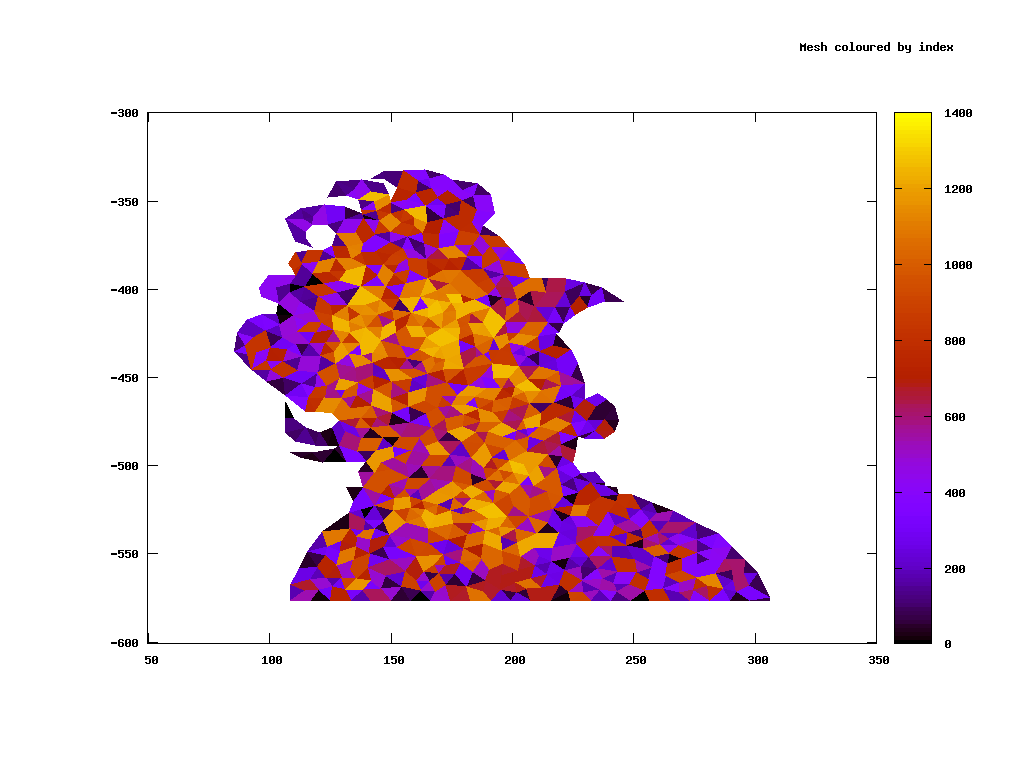
\includegraphics[width=.30\textwidth,height=.30\textwidth]{gnuplot_mesh_numbered}
}\subfigure[Analysis]{
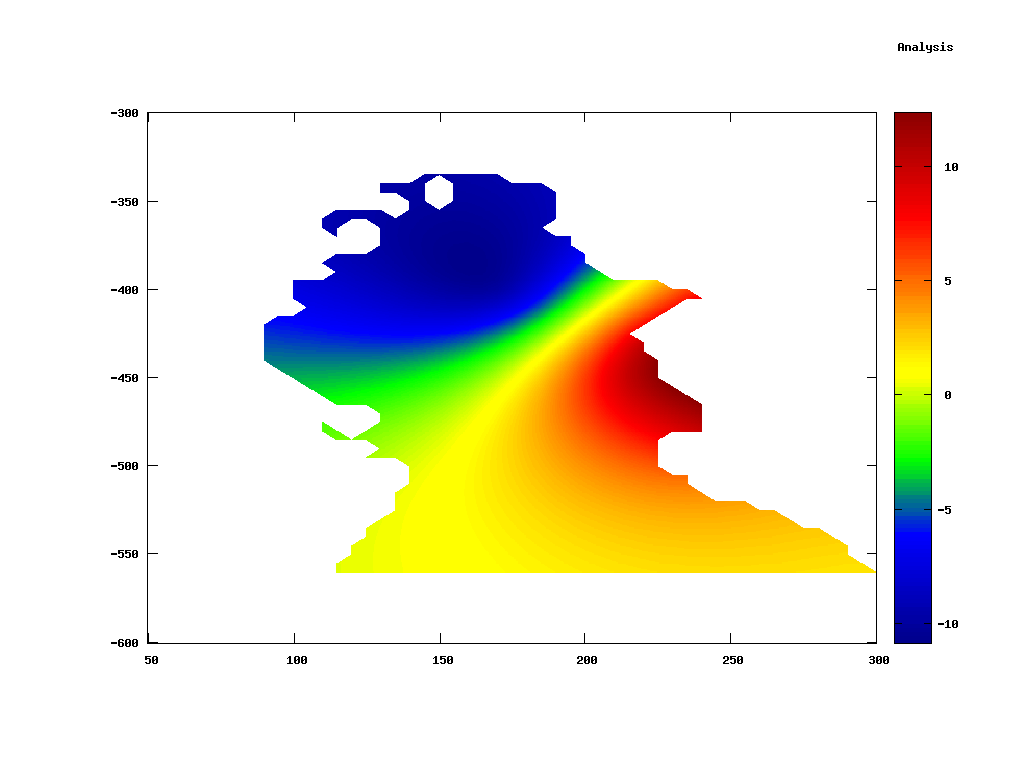
\includegraphics[width=.30\textwidth,height=.30\textwidth]{gnuplot_analysis}
}\subfigure[Error and data locations]{
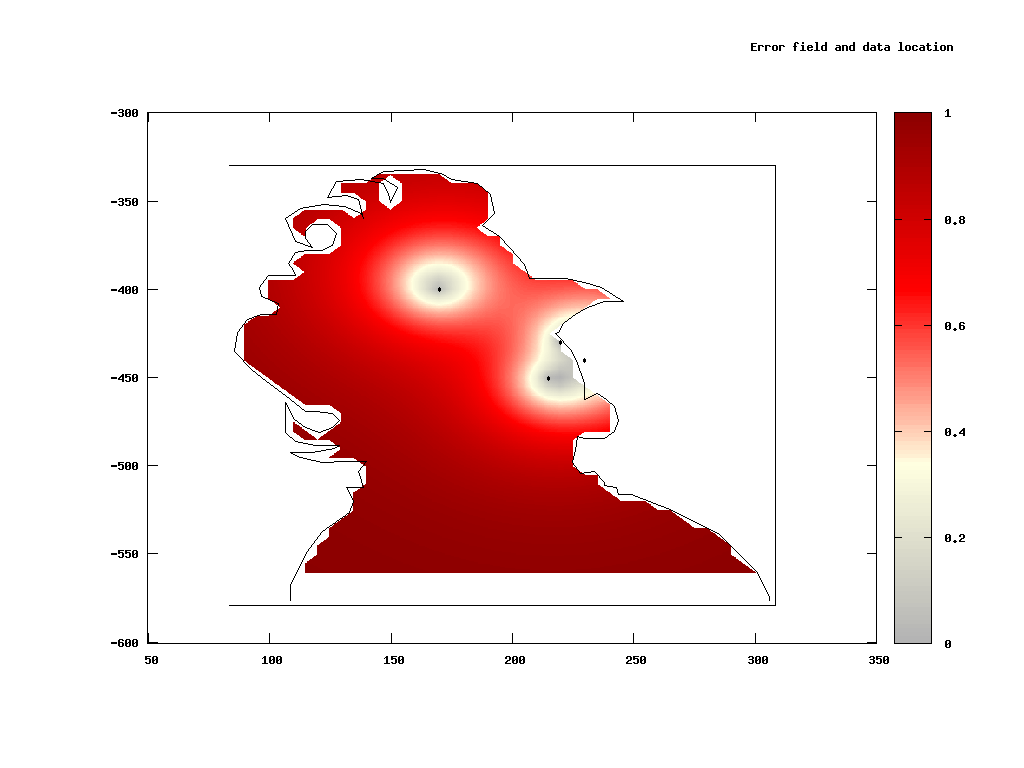
\includegraphics[width=.30\textwidth,height=.30\textwidth]{gnuplot_error_data}
}
\caption{Visualization with \gnuplot.\label{fig:gnuplotexamples}}
\end{figure}


\section{\matlab / Octave}
%-------------------

%http://modb.oce.ulg.ac.be/mediawiki/index.php/NetCDF_toolbox_for_Octave

\index{Matlab}
Tools to display contours, data, meshes, analysis and error fields are available at \url{http://modb.oce.ulg.ac.be/mediawiki/index.php/Diva_matlab}. 

\subsection{Installation}

In order to have the routines working properly, you need to installe:
\begin{description}
\item[NetCDF toolbox,] for reading the result files. For recent versions of \matlab, the routines for reading/writing NetCDF are readily available. For older versions, you can install it from \url{http://mexcdf.sourceforge.net/downloads/}.
\item[m\_map toolbox:] optional but recommanded, it allows one to plot generate various plots (mesh, data, analysis) using coastlines, projections etc. 
\end{description}
    

\subsection{Tools description}
%--------------------------

In most of the cases, you should only edit \texttt{diva\_start.m}, where you will define:

\begin{itemize}

\item the variable you want to plot:\\
\texttt{variable =} \begin{minipage}[t]{6.6cm}
            1 (temperature)\\
            2 (salinity)\\
            3 (depth)\\
            4 (velocity)\\
            5 (correlation length)\\
            0 (nothing)
           \end{minipage}
           
\item the path of your result and plot directories:\\

\texttt{dir.name} = name of your  \begin{minipage}[t]{3cm}    input/output \\  \command{divaload}/\command{divasave} \end{minipage}  directories called with\\
\texttt{dir.figures} = where you want figures to be saved.

\item the prefix of the figure names:\\  
    
\texttt{casename = 'Island';}

\item the figure format:\\

\texttt{fig\_format} = \begin{minipage}[t]{5cm}
           1 $\rightarrow$ jpeg\\
           2 $\rightarrow$ eps\\
           3 $\rightarrow$ png
           \end{minipage}
Matlab/Octave
\item the use of the \texttt{m\_map} package \footnote{\texttt{m\_map} is a mapping package for \matlab\, created and made available by Rich Pawlowicz at \url{http://www.eos.ubc.ca/~rich/map.html}} for your plots:\\

\texttt{is\_mmap} = \begin{minipage}[t]{5cm}
           1  if you have the \texttt{m\_map} toolbox installed;\\
           0  if not.
           \end{minipage}
\end{itemize}
 

Various scripts allow you to create plots, their purposes are self-explanatory for most of them:

\begin{enumerate}
\item \texttt{diva\_data.m},
\item \texttt{diva\_contour.m}, 
\item \texttt{diva\_mesh.m},
\item \texttt{diva\_analysis.m},
\item \texttt{diva\_error.m},
\item \texttt{diva\_data\_outliers.m}.
\end{enumerate}
\vspace{.25cm}

These six operations are summed in \texttt{diva\_plot\_all.m}. Along with these basic scripts, you also have at your disposal:
\begin{itemize}
\item \texttt{diva\_analysis\_mask.m} to plot the analysed field covered by a mask depending on the error field;
\item \texttt{diva\_contour\_depth.m} to plot all the contours generated through an execution of \texttt{divacont} (needs a \texttt{contour.depth} file to work);
\item \texttt{diva\_covafit.m} to plot the fitted and experimental covariance functions;
\item \texttt{diva\_inversetopo.m} to inverses the sign of the topography;
\item \texttt{diva\_topo.m} to plot topography using \texttt{topo.grd} file.
\end{itemize}

 
\btips
The provided \matlab\, scripts aim to show you how to create plots from files generated by \diva. Therefore do not hesitate to modify and adapt them to your own need.
\etips

\paragraph{Subroutines:} \texttt{uread.m} performs the reading of files written in GHER format (binary). These files are opened and closed with the help of \texttt{gzopen.m} and \texttt{gzfclose.m}, respectively. These three files do not need to be modified.


\subsection{Examples of plot with Matlab \diva toolbox}
%------------------------------------------------------------

\begin{figure}[H]
\centering
\subfigure[Data]{
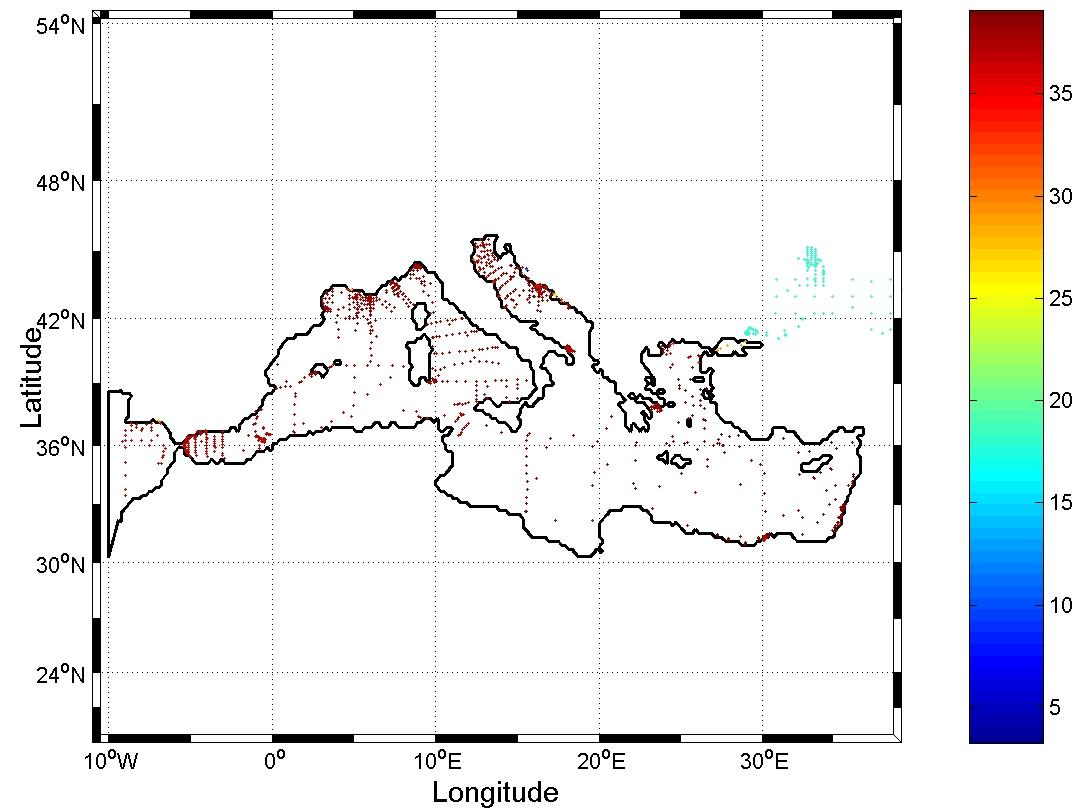
\includegraphics[width=.45\textwidth]{mat_data}
}\subfigure[Mesh]{
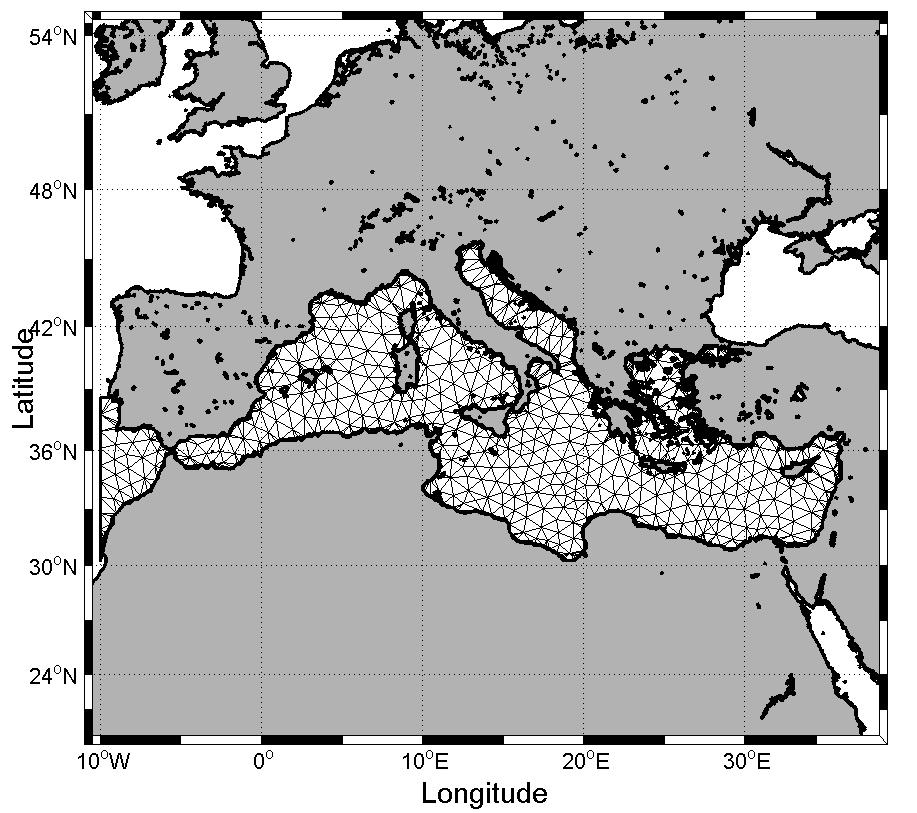
\includegraphics[width=.45\textwidth]{mat_mesh}
}
\subfigure[Analysis]{
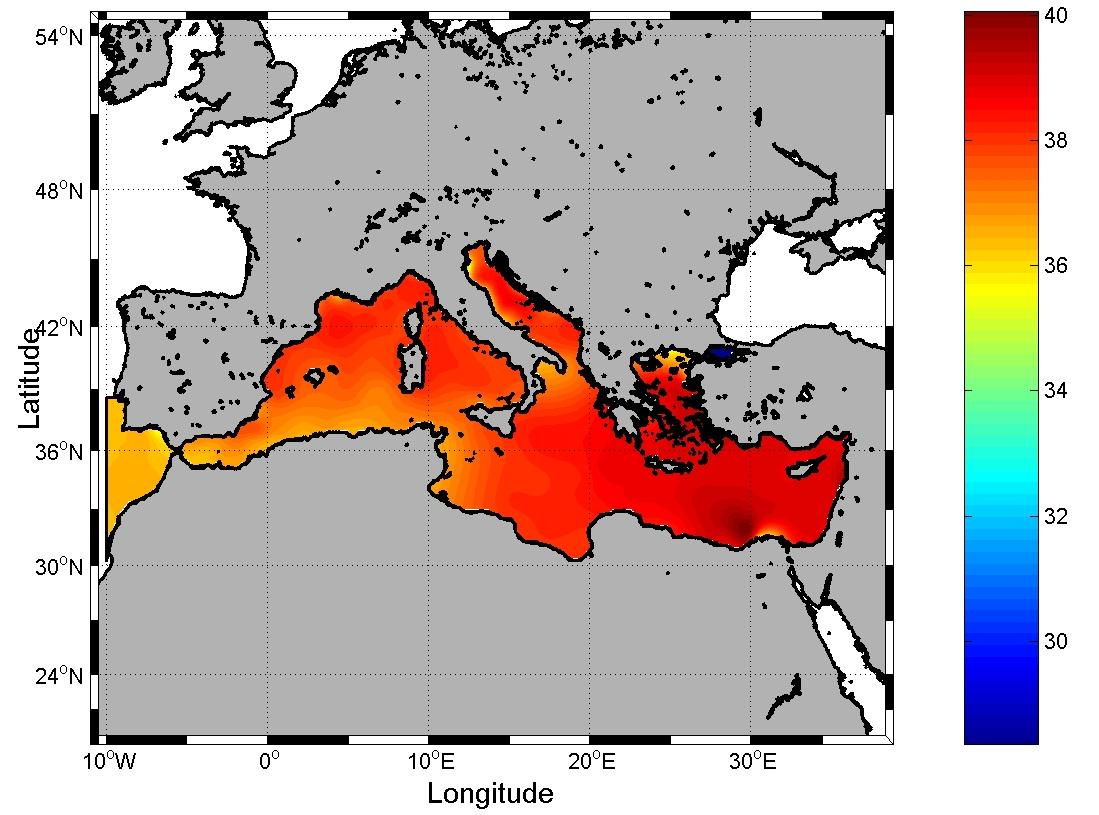
\includegraphics[width=.45\textwidth]{mat_analysis}
}\subfigure[Outliers]{
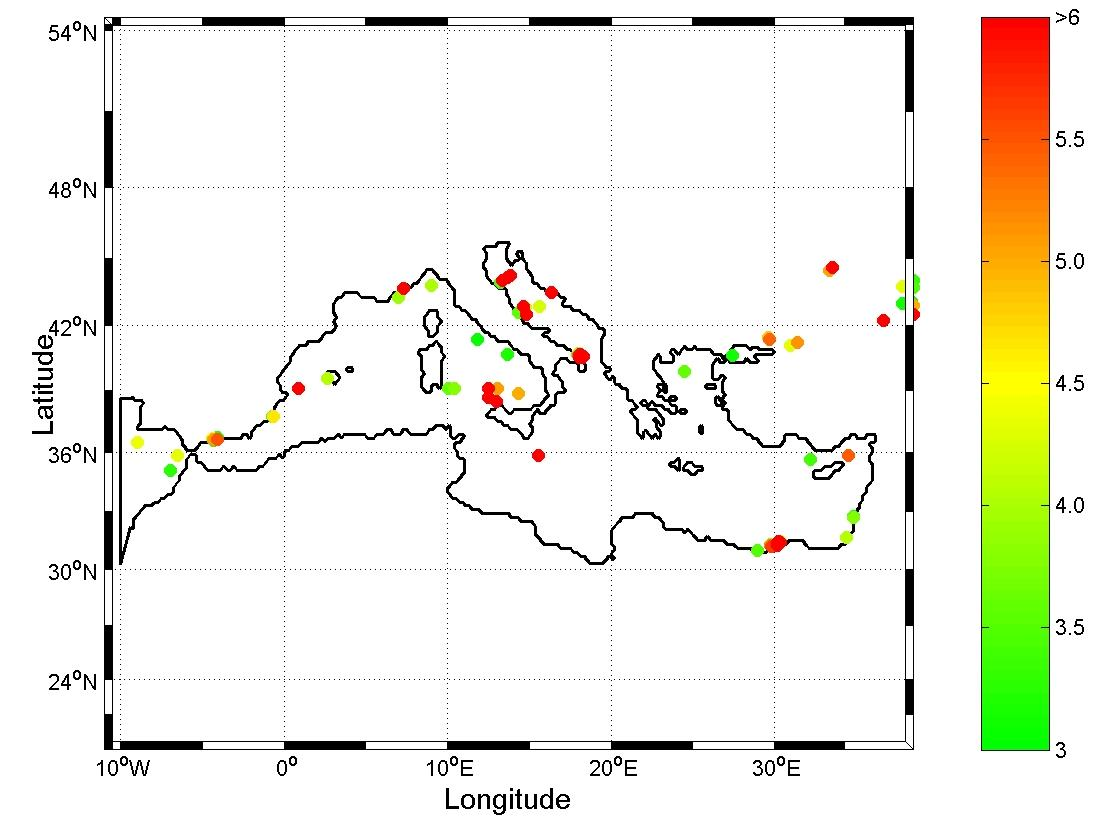
\includegraphics[width=.45\textwidth]{mat_outliers}
}
\caption{Examples of figures created with \matlab}
\end{figure}





\section{Python}
%_--------------


Python (\url{http://www.python.org/}) is a object-oriented, free to use, programming language. It is directly available through the package manager of recent Linux distributions.

\subsection{Installation}

Along with Python, it is necessary to install:
\begin{description}
\item[NumPy] \url{www.numpy.org}, a package for scientific computing;
\item[SciPy] (\url{http://www.scipy.org/}), another package for science and engineering;
\item[matplotlib] (\url{http://matplotlib.org/}), a 2D plotting library, where one can find the basemap toolkit (https://pypi.python.org/pypi/basemap) particularly useful for plot data on map projection (somewhat equivalent to m\_map in Matlab).
\end{description}

\subsection{Usage}


\section{General NetCDF visualization tools}
%---------------------------------------------

NetCDF (network Common Data Form) format. It is an machine-independent format to represent scientific data. For more details, consult \url{http://www.unidata.ucar.edu/software/netcdf/}. \index{NetCDF}

There are several tools that aim to provide a quick view of the content of a NetCDF files, such as the analyse and error fields provided by \diva. It is possible to export the results as a figure, but generally these software do not offer the possibility to customize the plots as could be done with the previous tools.

\subsection{NcBrowse}
%-------------------


\textsl{NcBrowse} is available at \url{http://www.epic.noaa.gov/java/ncBrowse/} and works with both Linux and Windows O.S.

\begin{figure}[htpb]
\centering
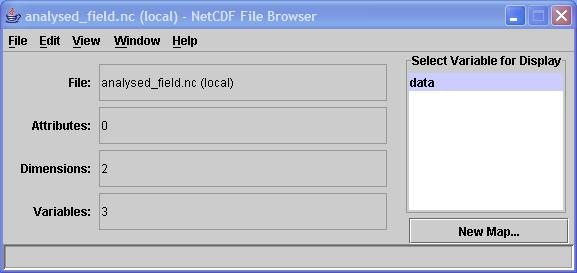
\includegraphics[width=.45\textwidth]{ncbrowse2}\hspace{.5cm} 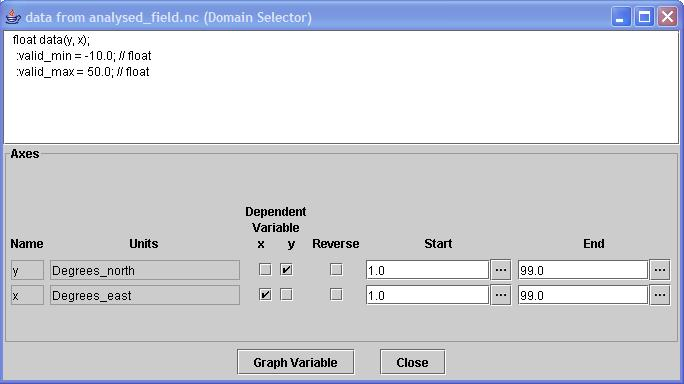
\includegraphics[width=.45\textwidth]{ncbrowse3} \\
\vspace{.5cm}
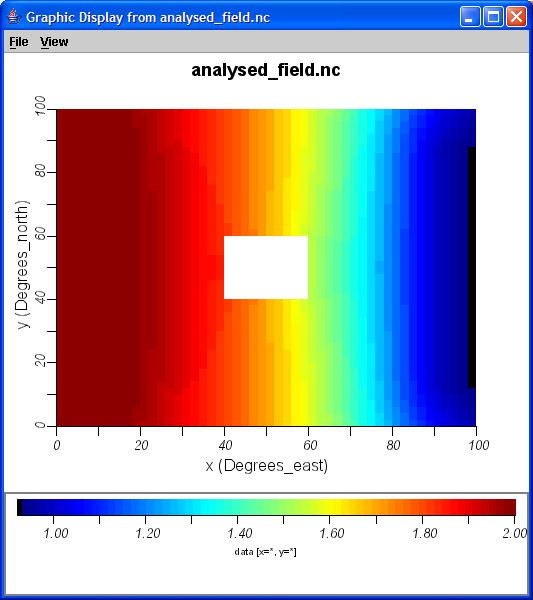
\includegraphics[width=.45\textwidth]{ncbrowse1} 
\caption{Plots of results with NcBrowse.}
\end{figure}

\subsection{Ncview}
%------------------

\index{Ncview}
\textsl{Ncview} (Linux and Windows + Cygwin) is available at\\
\url{http://meteora.ucsd.edu/~pierce/ncview_home_page.html}\\
but requires the NetCDF library to be compiled with your own system configuration.

\subsubsection{Installation under Linux}

Recent Linux distribution already permits the installation of Ncview through their package manager. Should it not be the case, the last version of Ncview is available here: \url{ftp://cirrus.ucsd.edu/pub/ncview/ncview-2.1.2.tar.gz}

\subsubsection{Installation under Windows-Cygwin}

Install and build the last NetCDF version for Unix: download the latest release and build as with Unix. The latest release is tested under Cygwin\index{Cygwin} and passes all tests cleanly. To build under Cygwin, follow the Unix build instructions in a Cygwin shell. The \texttt{--enable-shared} option to configure will generate the \file{netcdf.dll}. 


\begin{itemize}
\item Copy \url{http://www.unidata.ucar.edu/downloads/netcdf/netcdf-3_6_2/index.jsp}  into directory of your choice
\item Unzip the folder  and type:
\begin{lstlisting}[style=Bash]
[charles@gher13 Software]
./configure
...
make check..
...
make install
\end{lstlisting}

\item download \texttt{Ncview} and unzip the folder
\item type\\ 
\begin{lstlisting}[style=Bash]
[charles@gher13 Software]
./configure
...
make 
...
make install
\end{lstlisting}

\item type \texttt{startx} (check if you have installed \texttt{Xfree}) and in the newly opened window, type\\
\texttt{ncview name\_of\_the\_file.nc}

\item if the procedure is correctly followed, you should obtain windows similar to Fig.~\ref{fig:ncview}.
\end{itemize}

\begin{figure}[htpb]
\centering
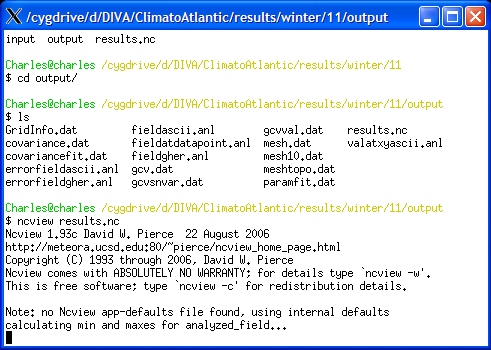
\includegraphics[width=.45\textwidth]{ncview0}\hspace{.5cm} 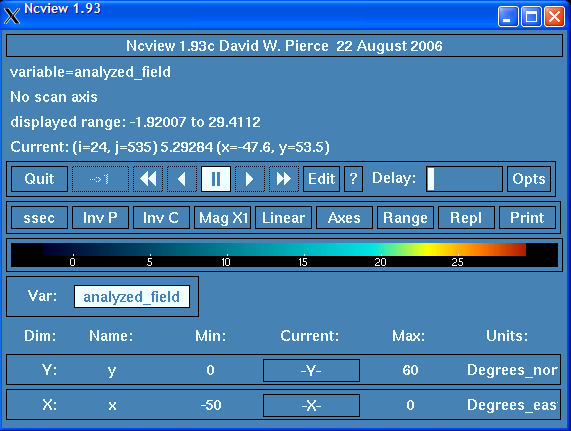
\includegraphics[width=.45\textwidth]{ncview1} \\
\vspace{.5cm}
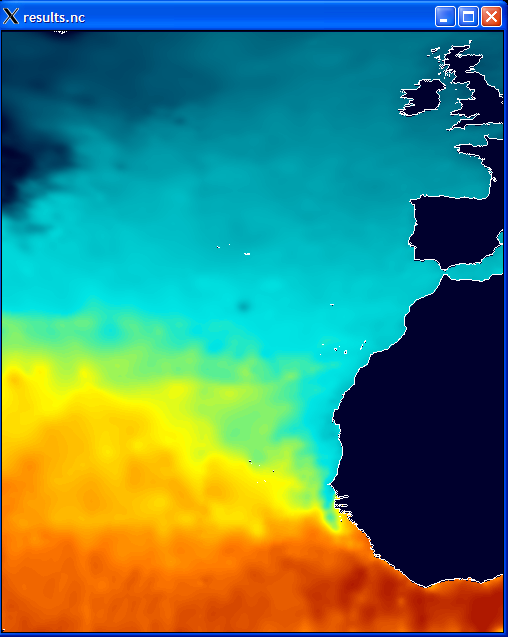
\includegraphics[width=.45\textwidth]{ncview2} \caption{Plots of results with \textsl{Ncview}.\label{fig:ncview}}
\end{figure}
